%%%%%%%%%%%%%%%%%%%%%%%%%%%%%%%%%%%%%%%%%
% Masters/Doctoral Thesis 
% LaTeX Template
% Version 2.5 (27/8/17)
%
% This template was downloaded from:
% http://www.LaTeXTemplates.com
%
% Version 2.x major modifications by:
% Vel (vel@latextemplates.com)
%
% This template is based on a template by:
% Steve Gunn (http://users.ecs.soton.ac.uk/srg/softwaretools/document/templates/)
% Sunil Patel (http://www.sunilpatel.co.uk/thesis-template/)
%
% Template license:
% CC BY-NC-SA 3.0 (http://creativecommons.org/licenses/by-nc-sa/3.0/)
%
%%%%%%%%%%%%%%%%%%%%%%%%%%%%%%%%%%%%%%%%%

%----------------------------------------------------------------------------------------
%	PACKAGES AND OTHER DOCUMENT CONFIGURATIONS
%----------------------------------------------------------------------------------------

\documentclass[
12pt, % The default document font size, options: 10pt, 11pt, 12pt
%oneside, % Two side (alternating margins) for binding by default, uncomment to switch to one side
english, % ngerman for German
singlespacing, % Single line spacing, alternatives: onehalfspacing or doublespacing
%draft, % Uncomment to enable draft mode (no pictures, no links, overfull hboxes indicated)
%nolistspacing, % If the document is onehalfspacing or doublespacing, uncomment this to set spacing in lists to single
%liststotoc, % Uncomment to add the list of figures/tables/etc to the table of contents
%toctotoc, % Uncomment to add the main table of contents to the table of contents
%parskip, % Uncomment to add space between paragraphs
%nohyperref, % Uncomment to not load the hyperref package
headsepline, % Uncomment to get a line under the header
%chapterinoneline, % Uncomment to place the chapter title next to the number on one line
%consistentlayout, % Uncomment to change the layout of the declaration, abstract and acknowledgements pages to match the default layout
]{MastersDoctoralThesis} % The class file specifying the document structure

\usepackage[utf8]{inputenc} % Required for inputting international characters
\usepackage[T1]{fontenc} % Output font encoding for international characters

\usepackage{mathpazo} % Use the Palatino font by default
\usepackage{amsmath}
\usepackage{mathtools}
\usepackage{amssymb}
\usepackage{graphicx}
\usepackage{rotating}
\usepackage[colorlinks=true, allcolors=blue]{hyperref}
\usepackage{url}
\usepackage[noend]{algpseudocode}
\usepackage{multirow}

\renewcommand{\vec}[1]{\mathbf{#1}}
\DeclareMathOperator*{\argmin}{arg\,min}
\DeclarePairedDelimiter{\norm}{\lVert}{\rVert}

\usepackage[backend=bibtex,style=ieee,natbib=true]{biblatex} % Use the bibtex backend with the authoryear citation style (which resembles APA)

\addbibresource{ref.bib} % The filename of the bibliography

\usepackage[autostyle=true]{csquotes} % Required to generate language-dependent quotes in the bibliography

%----------------------------------------------------------------------------------------
%	MARGIN SETTINGS
%----------------------------------------------------------------------------------------

\geometry{
	paper=a4paper, % Change to letterpaper for US letter
	inner=2.5cm, % Inner margin
	outer=3.8cm, % Outer margin
	bindingoffset=.5cm, % Binding offset
	top=1.5cm, % Top margin
	bottom=1.5cm, % Bottom margin
	%showframe, % Uncomment to show how the type block is set on the page
}

%----------------------------------------------------------------------------------------
%	THESIS INFORMATION
%----------------------------------------------------------------------------------------

\thesistitle{Estimation of abundances in microbial communities from metagenomic data} % Your thesis title, this is used in the title and abstract, print it elsewhere with \ttitle
\supervisor{Gregory \textsc{Kucherov}} % Your supervisor's name, this is used in the title page, print it elsewhere with \supname
\examiner{} % Your examiner's name, this is not currently used anywhere in the template, print it elsewhere with \examname
\degree{Labex Bézout Master's program in theoretical computer science} % Your degree name, this is used in the title page and abstract, print it elsewhere with \degreename
\author{Simone \textsc{Pignotti}} % Your name, this is used in the title page and abstract, print it elsewhere with \authorname
\addresses{} % Your address, this is not currently used anywhere in the template, print it elsewhere with \addressname

\subject{Computer Science} % Your subject area, this is not currently used anywhere in the template, print it elsewhere with \subjectname
\keywords{bioinformatics; metagenomics; abundance estimation; generalized linear models} % Keywords for your thesis, this is not currently used anywhere in the template, print it elsewhere with \keywordnames
\university{\href{http://www.u-pem.fr/}{Université Paris-Est Marne-La-Vallée}} % Your university's name and URL, this is used in the title page and abstract, print it elsewhere with \univname
\department{\href{http://ligm.u-pem.fr/}{Laboratoire d'informatique Gaspard-Monge}} % Your department's name and URL, this is used in the title page and abstract, print it elsewhere with \deptname
\group{\href{http://ligm.u-pem.fr/}{Labex Bézout Master's program}} % Your research group's name and URL, this is used in the title page, print it elsewhere with \groupname
%\faculty{\href{http://faculty.university.com}{Faculty Name}} % Your faculty's name and URL, this is used in the title page and abstract, print it elsewhere with \facname

\AtBeginDocument{
\hypersetup{pdftitle=\ttitle} % Set the PDF's title to your title
\hypersetup{pdfauthor=\authorname} % Set the PDF's author to your name
\hypersetup{pdfkeywords=\keywordnames} % Set the PDF's keywords to your keywords
}

\begin{document}

\frontmatter % Use roman page numbering style (i, ii, iii, iv...) for the pre-content pages

\pagestyle{plain} % Default to the plain heading style until the thesis style is called for the body content

%----------------------------------------------------------------------------------------
%	TITLE PAGE
%----------------------------------------------------------------------------------------

\begin{titlepage}
\begin{center}

\vspace*{.06\textheight}
{\scshape\LARGE \univname\par}\vspace{1.5cm} % University name
\textsc{\Large Rapport de Stage}\\[0.5cm] % Thesis type

\HRule \\[0.4cm] % Horizontal line
{\huge \bfseries \ttitle\par}\vspace{0.4cm} % Thesis title
\HRule \\[1.5cm] % Horizontal line
 
\begin{minipage}[t]{0.4\textwidth}
\begin{flushleft} \large
\emph{Author:}\\
\href{https://scholar.harvard.edu/simone_pignotti/home}{\authorname} % Author name - remove the \href bracket to remove the link
\end{flushleft}
\end{minipage}
\begin{minipage}[t]{0.4\textwidth}
\begin{flushright} \large
\emph{Supervisor:} \\
\href{http://www-igm.univ-mlv.fr/~koutcher/}{\supname} % Supervisor name - remove the \href bracket to remove the link  
\end{flushright}
\end{minipage}\\[3cm]
 
\vfill

%\large \textit{A thesis submitted in fulfillment of the requirements\\ for the degree of \degreename}\\[0.3cm] % University requirement text
%\textit{in the}\\[0.4cm]
\groupname\\\deptname\\[2cm] % Research group name and department name
 
\vfill

{September 2, 2018}\\[4cm] % Date
%\includegraphics{Logo} % University/department logo - uncomment to place it
 
\vfill
\end{center}
\end{titlepage}

%----------------------------------------------------------------------------------------
%	DECLARATION PAGE
%----------------------------------------------------------------------------------------

% \begin{declaration}
% \addchaptertocentry{\authorshipname} % Add the declaration to the table of contents
% \noindent I, \authorname, declare that this thesis titled, \enquote{\ttitle} and the work presented in it are my own. I confirm that:

% \begin{itemize} 
% \item This work was done wholly or mainly while in candidature for a research degree at this University.
% \item Where any part of this thesis has previously been submitted for a degree or any other qualification at this University or any other institution, this has been clearly stated.
% \item Where I have consulted the published work of others, this is always clearly attributed.
% \item Where I have quoted from the work of others, the source is always given. With the exception of such quotations, this thesis is entirely my own work.
% \item I have acknowledged all main sources of help.
% \item Where the thesis is based on work done by myself jointly with others, I have made clear exactly what was done by others and what I have contributed myself.\\
% \end{itemize}
 
% \noindent Signed:\\
% \rule[0.5em]{25em}{0.5pt} % This prints a line for the signature
 
% \noindent Date:\\
% \rule[0.5em]{25em}{0.5pt} % This prints a line to write the date
% \end{declaration}

% \cleardoublepage

%----------------------------------------------------------------------------------------
%	QUOTATION PAGE
%----------------------------------------------------------------------------------------

% \vspace*{0.2\textheight}

% \noindent\enquote{\itshape Thanks to my solid academic training, today I can write hundreds of words on virtually any topic without possessing a shred of information, which is how I got a good job in journalism.}\bigbreak

% \hfill Dave Barry

%----------------------------------------------------------------------------------------
%	ABSTRACT PAGE
%----------------------------------------------------------------------------------------

\begin{abstract}
\addchaptertocentry{\abstractname} % Add the abstract to the table of contents
Abstract
\end{abstract}

%----------------------------------------------------------------------------------------
%	ACKNOWLEDGEMENTS
%----------------------------------------------------------------------------------------

\begin{acknowledgements}
\addchaptertocentry{\acknowledgementname} % Add the acknowledgements to the table of contents
Gregory, Karel and Michael\\
Bézout
\end{acknowledgements}

%----------------------------------------------------------------------------------------
%	LIST OF CONTENTS/FIGURES/TABLES PAGES
%----------------------------------------------------------------------------------------

\tableofcontents % Prints the main table of contents

%\listoffigures % Prints the list of figures

%\listoftables % Prints the list of tables

%----------------------------------------------------------------------------------------
%	ABBREVIATIONS
%----------------------------------------------------------------------------------------

% \begin{abbreviations}{ll} % Include a list of abbreviations (a table of two columns)

% \textbf{LAH} & \textbf{L}ist \textbf{A}bbreviations \textbf{H}ere\\
% \textbf{WSF} & \textbf{W}hat (it) \textbf{S}tands \textbf{F}or\\

% \end{abbreviations}

%----------------------------------------------------------------------------------------
%	DEDICATION
%----------------------------------------------------------------------------------------

%\dedicatory{For/Dedicated to/To my\ldots} 

%----------------------------------------------------------------------------------------
%	THESIS CONTENT - CHAPTERS
%----------------------------------------------------------------------------------------

\mainmatter % Begin numeric (1,2,3...) page numbering

\pagestyle{thesis} % Return the page headers back to the "thesis" style

% Include the chapters of the thesis as separate files from the Chapters folder
% Uncomment the lines as you write the chapters


\chapter{Introduction}
\label{Chapter1}

\section{Context and Motivations}

Even before understanding the structure and function of DNA, humans have advanced hypothesis on how certain traits can be inherited over generations. While there is still much to be learnt about this molecule, the advent of molecular biology and bioinformatics marked the beginning of a new era, deeply changing people's perception of life. Technological advances enabled the analysis of DNA and other biological molecules, whose sequences can now be observed and for which we found a convenient representation as strings over a small fixed alphabet. Such representation enables their computational analysis, often using algorithms which were originally conceived for the analysis of text.

Starting from simple microbial organisms, researchers started to assemble the short genomic sequences produced by sequencing technologies into genes and chromosomes, till the entire human genome has been characterized in 2001. Nowadays, genomic databases like NCBI's GenBank contain billions of sequences, and in the case of GenBank its size is doubling approximately every 18 months \footnote{~\url{https://www.ncbi.nlm.nih.gov/genbank/statistics/}}. Several algorithmic challenges were introduced by the amount of sequencing data being generated, spanning from compression and storage to annotation and comparison.

The incredible amount of information stored in these sequences is far from being extracted. Algorithmic challenges and technological limitations make the comprehensive analysis of all the produced sequencing data impossible at the current state, and including every such sequence in a genomic ``search engine'' is unfeasible even with the latest methods and the advances in cloud computing. The potential of these data for understanding human diseases and environmental issues is astonishing, and there is a real need for the development of efficient algorithms and data structures for this most relevant field of Big Data.

Nevertheless, progress in bioinformatics created the possibility to study entire populations and communities of hundreds of different microbial species without the need to isolate single clonal populations or cells. In metagenomics, the genetic material extracted from environmental samples is sequenced and the resulting short fragments of DNA, called \textit{reads}, are assigned to an extensive database of reference genomes. The size of the datasets, the mutations occurring at a fast pace and the presence of organisms which have never been sequenced yet make the use of standard mapping algorithms not fit for this scenario. Therefore new methods are being developed which carry out the task of assigning short sequences to the genomes of the organisms they are most likely to be originated from, using heuristics for speeding up the computation, decreasing the space complexity and estimating the composition of the sample.

Here we focus on the estimation of relative abundances of microbial organisms in metagenomic samples, and we introduce a method to probabilistically distribute the assignments of the metagenomic classifiers, in particular those of our software ProPhyle. We use a linear regression model to account for the similarities of the reference genomes and solve the problem of reads which map equally well to multiple reference genomes. We show that the method provides accurate results and is comparable to other state-of-the-art abundance estimation tools.

In the rest of this chapter we introduce notions about the analysis of genomic sequences and we provide a background for readers who are not keen to bioinformatics. In Chapter \ref{Chapter2} we analyze relevant programs and algorithms performing both read assignment and abundance estimation. In Chapter \ref{Chapter3} we introduce the method we propose and finally in Chapter \ref{Chapter4} we show the results obtained on different datasets.

\section{Analysis of DNA sequences}

% NGS data
Even though they may sound like fairly simple organisms, the genomes of most bacterial species are composed of millions of nucleotides. Obtaining a faithful representation of them is until today a big challenge, mostly because modern sequencing technologies only provide short fragments (\textit{reads}) of this long chain, usually in the order of few hundred base pairs, or letters; while cutting-edge tools may produce longer sequences, this is at the cost of introducing a considerable amount of sequencing errors. In both cases, reads need to be assembled like puzzles to recover the original genome of the organism, a task which requires a good coverage of the genome and that is made more complex by the presence of highly repetitive portions called \textit{low-complexity regions}. In reference-based metagenomics, a database of high quality reference genomes is needed for the assignments not to be biased by i.e. contamination from other organisms or poor assembly.

% Sequence Alignment
Indeed, the reads of the metagenome need to be compared to a set of reference genomes in order to estimate the composition of the sample. The first algorithms to perform the comparison of two sequences were based on dynamic programming: the input sequences were aligned in such a way to minimize the number of mismatches, insertions or deletions to transform one sequence into the other. These algorithms soon became computationally unfeasible due to the fact that unforeseen amounts of data were being generated, that they only allowed pairwise comparison, and that their cost was quadratic in the size of the input sequences. In the current setting, the analysis of metagenomic reads with such a tool would require years; furthermore, the actual alignment is not needed to assess the composition of the sample, and we are mainly interested in which genome the read is originated from.

% Alignment Free
Soon heuristic methods were developed for sequence comparison, whose BLAST is probably the best representative and is therefore analyzed in Chapter \ref{Chapter2}. Most importantly, the alignments are performed only for those reference genomes which have an exact match for a subsequence in the read, drastically reducing the number of pairwise comparisons. In the context of metagenomics though, even tools like BLAST, which are still used in other omics fields, became unfeasible for the current size of experiments. Pushing the idea behind BLAST's so-called ``\textit{seed-and-extend}'' paradigm, alignment-free algorithms started to take its place. In alignment-free sequence comparison, sequences are viewed as sets of substrings of fixed size $k$, called $k$-mers, which can be indexed and queried promptly. Reads are then assigned to genomes sharing enough $k$-mers with them. This similarity measure, surely weaker than alignment score, allows the analysis of huge metagenomic samples in a fraction of the time: as an example, the software Kraken (also analyzed in Chapter \ref{Chapter2}) reaches assignment speeds of up to a million reads per minute on databases containing thousands of reference genomes.

This performance is achieved also thanks to the organization of sequences in an evolutionary tree reflecting sequence similarity, called \textit{phylogenetic} tree, which is commonly used in metagenomics to compress the references and provide abundance estimates at different level of the tree. A special kind of phylogenetic tree, called \textit{taxonomic} tree, is often used as it contains annotations like names for different levels of the tree, reflecting the characteristics of the subtree (i.e. species, genera, families). Since genomes in the same species share most of their genetic material, reads may now be assigned to internal nodes of the tree; furthermore, biological mechanisms like horizontal gene transfer, allowing bacteria of different species to exchange portions of their DNA, make assignments even more complex since a short read fragment may match equally well reference genomes associated to distant leaves of the tree.

%Estimation of Abundances
Estimating abundances solely from the unique mappings to the references has been shown to introduce considerable biases \cite{lu_bracken:_2017} due to the uneven representation of microbial clades in the genetic databases and their variable average similarity within those clades. Therefore methods have been developed to probabilistically redistribute assignments to multiple reference genomes or to internal nodes of the taxonomic tree to fixed ranks, like species or genus. While these methods approximate very closely the abundances of the samples at such ranks, they once again introduce biases linked to the structure of the tree, which is constant subject of discussion and dissent in the microbiology community. For this reason, and to provide better resolution to the results, modern tools focus mainly on the genome level.


\chapter{State of the Art} % Main chapter title
\label{Chapter2}

In this chapter we present some of the tools which had a big impact in the field of bioinformatics, and especially metagenomics. Even though we focus on abundance estimation techniques, we provide an overview of the most important methods for the assignment of reads, both based on alignments and on $k$-mer composition, since their properties highly influenced the solutions adopted for the actual estimation of abundances. This list is not nearly extensive, and we refer to \textbf{[ref karel]} for a more detailed overview, especially for read assignment.

\section{Read Assignment}

\subsection{Alignment-based Methods}

\subsection{Alignment-free Methods}

\section{Abundance Estimation}

\subsection{Expectation-Maximization}

\subsection{Generalized Linear Models}

\subsection{Bayesian Re-estimation}
 

\chapter{Methods}
\label{Chapter3}

\section{Context}

To cope with the complexity of metagenomes, the size of the reference databases and the resulting uncertainty in read assignments, early abundance estimation tools like \textbf{[ref bracken]} and \textbf{[ref megan]} did not provide the abundances for each reference genomes, but only for taxonomic clusters like species, genus or phylum.

This approach introduces a bias due to the structure of the phylogenetic or taxonomic tree, in which some species may be over-represented, others are still subject to adjustments, and in certain cases the definition is not coherent: in the Mycobacterium genus, for instance, Mycobacterium Bovis and Mycobacterium Tuberculosis are classified as two different species even though their genomes are characterized by 99.5\% similarity, while the threshold used for species separation is usually 97\% \textbf{[ref myco]}.

Furthermore, the technological improvements in read sequencing provide increased resolution for the metagenomic samples, by generating either short high quality reads with error rate <1\% as with Illumina and Sanger machines, or long reads with higher error rates as with ONT and PacBio. The detail of the information in these sequences allow, with sufficiently high coverage, to map at least some of the reads in the metagenome to the exact reference genome they are likely to come from, when they are present in the database.

Nevertheless, due to the high similarity among the reference genomes of the same species, most reads, especially those associated to the core genome, will still map to multiple references equally well. Therefore reads assigned to subsets of the reference database need to be probabilistically redistributed to each genome.

Several tools including Bracken and GASiC build their model for read redistribution on top of the estimated similarity of the reference genomes. In Bracken \textbf{[ref bra]}, every $k$-mer of each reference is mapped to the index using the Kraken algorithm, and the frequency with which $k$-mers are assigned to internal nodes of the taxonomic tree are used to estimate the probability that a read of the metagenome assigned to such internal nodes originates from each reference in its subtree using Bayes' theorem. In this model, the $k$-mer length $k$ should match the length of the reads in the sample, but the technology used to sequence the metagenome is not taken into account, reducing the robustness of the method. By fixing $k$, it also makes it unfit for machines producing reads of variable length like ONT. Furthermore, by assigning every $k$-mer of the database it increases the computational burden and the risk of overfitting.
Gasic \textbf{[ref gas]} introduced a new approach based on read simulation. Read simulators provide realistic sequences by using probabilistic models built from the results of different sequencing technology. This allows the abundance estimation to be independent from the sequencing technology, which evolves at a fast pace. Reads are simulated from each reference genome with a low coverage and with parameters resembling those of the metagenomic sample, then aligned to the references using a fast aligner like BWA \textbf{[ref bwa]} or Bowtie \textbf{[ref bow]}. Reads mapped to multiple reference genomes are used to build a similarity matrix which is specific to the sequencing technology and the aligner used in the real experiment, and a LASSO linear model is built on top of it \textbf{[ref las]}.

Inspired by these two methods, we developed an abundance estimator for alignment-free tools, which has been integrated in the program ProPhyle. Exploiting ProPhyle's lossless $k$-mer index, producing assignments which are more accurate than Kraken's (see figure \textbf{[ref fig]}), we decided to focus on the genome level and to make use of the model introduced by Gasic for alignment tools.

\subsection{Desired Properties}

A major problem with Bracken and other abundance estimators is the amount of false positives in their output. Indeed, due to the size of modern metagenomic read sets, which may contain up to billions of sequences, it happens frequently that reference genomes which are known not to be present in the sample still have non-zero assignment counts. This happens either because those genomes are highly similar to other references which indeed are present in the sample, or because those reads are generated from a novel strain which is not included in the database and has no better representative, in which case the assignment will probably have a low score.

While dealing with the second issue requires a preprocessing step to filter out poor quality assignments, the first one can be solved by defining thresholds for the number (or percentage) of specific assignments that a given genome needs to get to be considered as present, where specific means that no other reference genome is matched equally well, as it is done in Bracken. Nevertheless, this solution is once again affected by the uneven representation of species in the database, where well-studied species like human pathogens include hundreds or thousands of representative genomes while others only have few representatives. In the first case, the probability that a read matches an exact genome instead of an entire cluster decreases considerably, since most $k$-mers are shared by the whole cluster.

The solution adopted in Gasic, using LASSO to regularize the linear redistribution model and filter out false positives, also has some drawbacks. The major issue appears in the presence of highly similar clusters in the reference database: if the genomes in the cluster all have a comparable amount of assignment, the $L_1$ regularization penalty will be likely to select one of them at random and filter out the others.

To address the issue of Gasic, we used the Elastic Net regressor. Elastic Net combines the $L_1$ regularization used in LASSO and the $L_2$ regularization (also called Tikhonov or Ridge regularization). We will show that the Elastic Net can be seen as a generalization of LASSO, and that it introduces a so-called ``grouping effect'', avoiding the random selection of highly correlated genomes as it happens with LASSO. Furthermore, the path with which predictors are set to 0 by its variable selection property is more stable than LASSO's when regularization parameters change. This feature guarantees consistent results when using different parameters to fit metagenomes of different complexity.

\subsection{Linear Regression}

Linear regression is a linear approach to modelling the relationship between a scalar response (or dependent variable) and one or more explanatory variables (or independent variables) \textbf{[ref wiki]}. The relationship between these two sets of variables is modeled with linear functions of the kind:
\begin{equation*}
    y_i = \beta_0 + \beta_1 x_{i1} + \dots + \beta_p x_{ip} + \varepsilon_i ~,~~ i = 1, \dots , n
\end{equation*}
where $y_i$ is the response variable, the vector $\vec{x_i} = \{x_i1, \dots, x_ip \}$ contains the $p$ explanatory variables for $y_i$, the vector $\boldsymbol{\beta} = \{\beta_0, \dots, \beta_p \}$ is the vector of regression coefficients including the intercept term $\beta_0$, and $\varepsilon_i$ is an error term which accounts for noise in the data. In matrix notation, the model can be expressed as:
\begin{equation*}
    \vec{y} = \boldsymbol{X}\boldsymbol{\beta} + \boldsymbol{\varepsilon}
\end{equation*}

The standard method for estimating the regression coefficients is Ordinary Least Squares (OLS). This method consists in minimizing the sum of the squares of the differences between the observed dependent variable and those predicted by the linear function \textbf{[ref wiki]}. This is equivalent to the optimization of the following function:
\begin{equation*}
    \boldsymbol{\hat{\beta}} = \argmin_{\beta}{\norm{\vec{y} - \boldsymbol{X}\boldsymbol{\beta}}_2^2}
\end{equation*}
Under the assumption that the error vector $\boldsymbol{\varepsilon}$ is normally distributed, OLS is therefore equivalent to the Maximum Likelihood (ML) estimator \textbf{[ref wiki]}.

In the context of metagenomic abundances, the observed assignment counts can be modelled as the dependent variables of a linear model, while the regression coefficient could represent the unknown abundances of the reference genomes in the sample, to be estimated using some explanatory matrix. In our case, the explanatory variables will be measures of similarity of the reference genomes. Due to the similarities between genomes of the same species being very high, and to the increasing number of genomes used as references in metagenomic experiments, it is unrealistic to expect this model to fit the data by simply using OLS. In fact, in this case most of the genomes will be considered as present by the model, since the reads in the sample will be mapped to several references, but only few of them will actually be present. To address this issue, we use a model which performs both regularization and variable selection: the Elastic Net.

\subsection{The Elastic Net}

To avoid overfitting a linear model, or to improve its performance when the problem is ill-posed, the technique of regularization is often used. In a regularized model, a regularization term is included in the minimization we have already seen for OLS:
\begin{equation*}
    \boldsymbol{\hat{\beta}} = \argmin_{\beta}{\norm{\vec{y} - \boldsymbol{X}\boldsymbol{\beta}}_2^2} + \norm{\boldsymbol{\Gamma}\boldsymbol{\beta}}_2^2
\end{equation*}
where $\boldsymbol{\Gamma}$, called Tikhonov matrix, is usually chosen as a multiple of the identity matrix. Although introducing this $L_2$ regularization penalty, so called because it uses the $l^2$ norm or Euclidean distance, has a beneficial effect on overfitting issues by shrinking large regression coefficients, an $L_1$ regularization penalty can be used in order to enforce their sparsity, thus performing variable selection. This technique, known as LASSO \textbf{[ref lasso]}, has been already proved to be an effective solution for metagenomics in \textbf{[ref gasic]}.

While the most intuitive way to enforce sparsity is by using the $l^0$ norm, i.e. the number of non-zero coefficients, this would break the convexity of the objective function to optimize, making it an NP-hard problem \textbf{[ref convex]}. Nevertheless, the $l^1$ norm has been shown to approximate $l^0$, therefore providing similar performance without loosing the convexity property.
On the other hand, the $l^2$ norm does not provide the same effect: the intuition of the reason is in the figure \textbf{[L1-L2]}. Let us consider the problem as a constrained optimization problem:
\begin{equation*}
    \boldsymbol{\hat{\beta}} = \argmin_{\beta}{\norm{\vec{y} - \boldsymbol{X}\boldsymbol{\beta}}_2^2}~~\text{s.t.}~~f(\beta) \leq t
\end{equation*}
for $f=\norm{\cdot}_1$ and $f=\norm{\cdot}_2^2$. In the first case, the likelihood of a convex object which lies tangent to the boundary to encounter a ``corner'' is higher than in the second case, where the rotational invariance of the ($n$-)sphere contrasts this property. Figure \textbf{[ref fig]} gives an intuition of this in the 2-dimensional space.

\begin{figure}
  \caption{Optimization space for the $L_1$, $L_2$ and Elastic Net regularizations in 2D.}
  \centering
    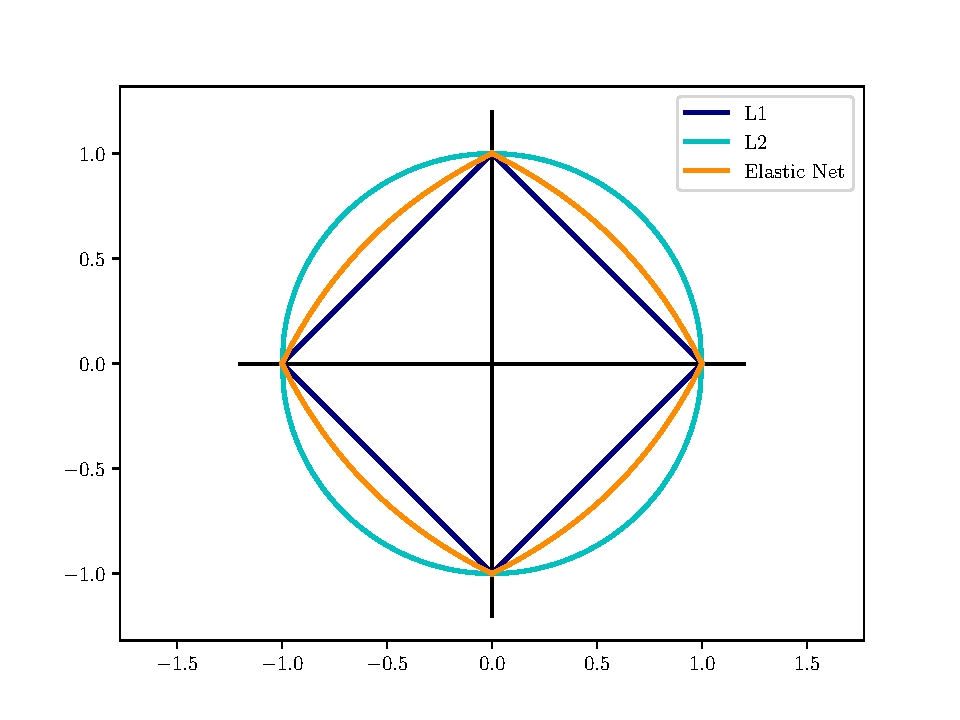
\includegraphics[width=1\textwidth]{Figures/reg_norms.pdf}
\end{figure}

\begin{figure}
  \caption{Example of regularization path for the coefficients of the LASSO and Elastic Net methods on the same instance. Varying the regularization weight $\alpha$ results in smoother transitions for the Elastic Net.}
  \centering
    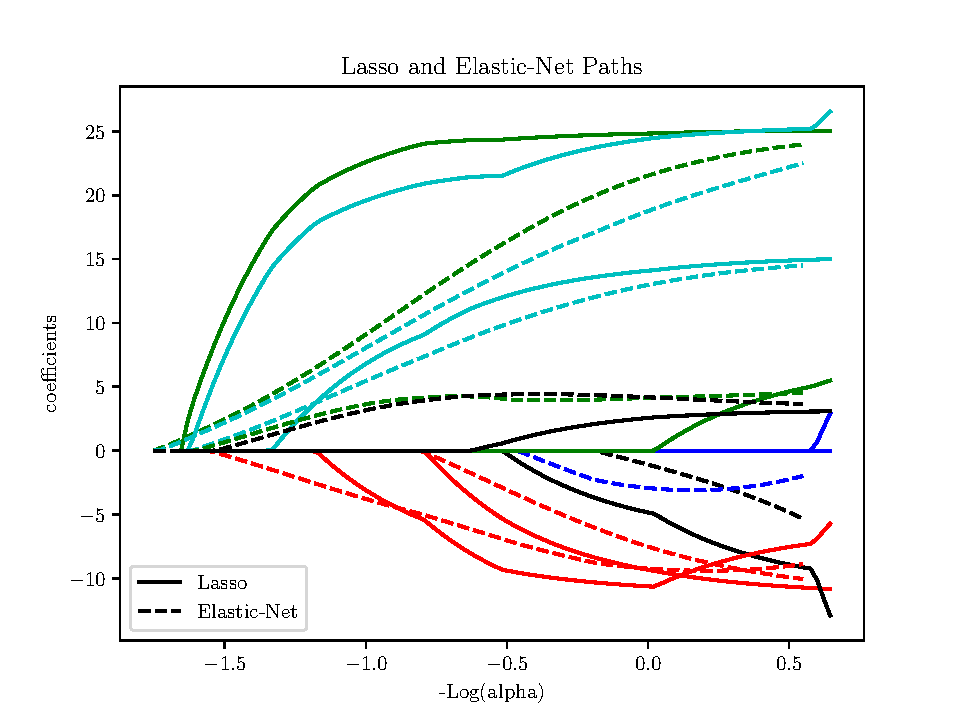
\includegraphics[width=1\textwidth]{Figures/enet_vs_lasso.pdf}
\end{figure}

While both $L_1$ and $L_2$ regularization penalties have desirable properties for our application, respectively the sparsity and the shrinking of the regression coefficients, they both come with some drawbacks. The LASSO has been shown to be extremely variable because of its inherent discreteness, as shown in \textbf{[ref Breiman and enet]}. On the other hand, the Tikhonov regression does not provide the desired variable selection property, since using the $l^2$ norm it keeps all the predictors in the model. It has also been observed that in a variety of applications, each technique may perform better than the other.

The Elastic Net addresses the issues above by linearly combining the $L_1$ and $L_2$ regularization penalties. The resulting objective function to optimize is:
\begin{equation*}
    \boldsymbol{\hat{\beta}} = \argmin_{\beta}{\norm{\vec{y} - \boldsymbol{X}\boldsymbol{\beta}}_2^2} + \lambda_1 \norm{\boldsymbol{\beta}}_1 + \lambda_2\norm{\boldsymbol{\beta}}_2^2
\end{equation*}

The greatest advantage provided by this method is its grouping effect. As shown in Theorem 1 of \textbf{[ref enet]}, this property tends to give similar regression coefficients to highly correlated variables. This is particularly important when fitting metagenomic data of high complexity, where several strains of the same species may be present in the sample. In such situation, LASSO would be likely to only select one such variable at random \textbf{[ref enet]}.

\subsection{Solving Linear Models}
\begin{itemize}
    \item coordinate descent
    \item SVM reduction
\end{itemize}
A technique frequently used for solving linear models, including the sklearn python library implementation we use for the benchmarks of this model, is coordinate descent. Coordinate descent algorithms fix the majority of components in the regression coefficients vector at their value from the current iteration, and approximately minimize the objective function for the non-fixed coordinates. The subproblems are of lower dimension, thus easier to solve than the original problem \textbf{[ref cd]}. These algorithms are especially fit for computational statistics and machine learning applications, where the cost of computing one component of the gradient is low and there is no need for extreme accuracy.

\begin{itemize}
    \item algo for regularization term
    \item cyclic vs random
\end{itemize}

\section{Model}

Inspired by the LASSO linear model defined in \textbf{[ref gasic]} and the improvements in its successor \textbf{[ref ditasic]}, we have designed a model to estimate metagenomic abundances from read assignments, focusing especially on the properties of the assignments of the metagenomic classifier ProPhyle.

Thanks to the lossless property of ProPhyle's index, its read assignments have a higher resolution than other alignment-free methods (cf. \ref{Chapter2}). Even though metagenomic reads can still be assigned to internal nodes of the taxonomic tree, this has a different meaning with respect to the assignments of e.g. Kraken: for ProPhyle, a read is assigned to an internal node if and only if every genome in its subtree has the same assignment score (i.e. shares the same number of $k$-mers with the read); for Kraken, this may happen if two or more, possibly distant genomes have the same score, in which case the tie would be solved by assigning the read to their lowest common ancestor (LCA) instead of providing their list, or if they share every $k$-mer in the read, in which case the $k$-mers themselves would be associated to their LCA in the database, making a precise assignment impossible in the first place.

Therefore we designed a model which focuses on the genome level, and which does not take into account the structure of the taxonomic tree but only the actual similarity of the reference genomes, as it is ``perceived'' through ProPhyle's index and assignment algorithm. As introduced in \textbf{[ref gasic]}, a first simulation step is performed in order to estimate such similarities, then read assignments are optimized using an Elastic Net-based linear model.

\subsection{Model Definition}

\subsubsection{Similarity matrix estimation}
In order to estimate the similarity between each couple of reference genomes, reads are simulated from each of them and assigned to the full reference set. The similarity matrix, whose columns encode the distribution of the assignments, is built as follows:
\begin{algorithmic}
\State $\mathbf{S} \gets \mathbb{M}_{n\times n}$
\For {ref. genome $i \in D$}
\State $s_{*i} \gets \mathbf{0}^n$
\State simulate read set $R_i$ from genome $i$
\For {read $\in R_i$}
\State $I \gets$ assign(read)~~~[$I \subseteq D_n$]
\For {$j \in I$}
\State $s_{ji}~~{+=}~~1$
\EndFor
\EndFor
$s_{*i}~~{/=}~~s_{ii}$
\EndFor
\end{algorithmic}
where $D_n$ is the reference database containing the $n$ reference genomes.

The value of $s_{ij}$ encodes the number of reads simulated from reference $j$ which map to reference $i$, divided by the number of reads which map back to a subset containing reference $j$. This represents an estimate for the similarity of genomes $(i,j)$, according to their $k$-mer composition encoded in the ProPhyle index used for the assignment.

\subsubsection{Optimization}
Let $\vec{m} = [m_1, \dots, m_n]^T$ be the vector of mappings of a sample, calculated in the very same way as a column of $\boldsymbol{S}$ (its sum will exceed the total number of reads in the sample, since a multiple assignment to subset $I$ will increment by 1 the entry of each reference genome $g_j \in I$). In order to recover the vector of true abundances $\mathbf{r} = [r_1, \dots, r_n]^T$, we need to solve the following system of linear equations:
\begin{equation*}
  \vec{m} = \boldsymbol{S} \cdot \vec{r}
\end{equation*}
with non-negativity constraints $r_i \geq 0~\forall i$. The equation corresponding to genome $i$ is:
\begin{equation*}
  m_i = r_i + \sum_{i \neq j}^n s_{ij} \cdot r_j
\end{equation*}

To estimate the solution to this system, we solve it using $\vec{r}$ as the regression coefficient vector of the Elastic Net.

\subsection{Implementation}

Simulating reads which reflect the properties of the metagenomic sample to be classified is a crucial step of the optimization pipeline: parameters like read length and error profile of the technology used to sequence the real sample may highly affect the performance of the method. For this reason, we have used the simulation framework RNFsim \textbf{[ref rnf]} in the implementation of this step. RNFsim includes some of the most efficient and accurate read simulators and enables reproducible and fully-parametrizable read simulation; it can also easily be extended to match the characteristics of evolving sequencing technologies. In order to obtain accurate results, the simulated reads should match the characteristics of the real data as closely as possible.

For the optimization step, we relied on the implementation of the coordinate descent algorithm for Elastic Net provided by the scikit-learn Python framework. The code\footnote{\url{https://github.com/scikit-learn/scikit-learn/blob/master/sklearn/linear_model/cd_fast.pyx}} which performs the optimization is implemented in C as a Cython extension, and provides fast and stable convergence as showed in \ref{Chapter4}.

At the time of writing, all the programs and scripts are publicly available in ProPhyle's Github repository\footnote{\url{https://github.com/prophyle/prophyle}} in the branch \texttt{enet\_abundances}. Every step in the pipeline described above will be integrated in the next main release of ProPhyle.

\subsection{Error estimations}

To benchmark the method we used the two following error measures, where $e_i$ and $t_i$ are respectively the estimated and true abundances of genome (or species, genus, etc.) $i$:
\begin{itemize}
  \item MAE (Mean Absolute Error):
  \begin{equation*}
    \frac{\sum_{i=1}^n |e_i - t_i|}{n}
  \end{equation*}
  \item RSS (Residual Sum of Squares):
  \begin{equation*}
    \sum_{i=1}^n (e_i - t_i)^2
  \end{equation*}
\end{itemize}

In addition to these measures of the distance between the true and estimated abundances, we focused on the false positive and false negative rates, which are arguably the most important measures in many metagenomic experiments: while slight changes in the relative abundances may be interesting for some particular applications, having a reliable list of what the sample is composed of is always a valuable information. Furthermore, we provide two measures for those rates: first, the number of FP (resp. FN), i.e. the amount of genomes which are present in the output of the programs but not in the sample (resp. present in the sample and not in the output), and secondly their relative abundance. We will show that our method achieves superior genome selection performances with respect to the other tools analyzed, while improving the error calculated with the measures above.


\chapter{Results and Discussion} % Main chapter title
\label{Chapter4}

\section{Results}

To evaluate the performance of this abundance estimation framework, we used both a simulated readset, in which the reference genome generating each read is known and the exact abundances are ,

\subsection{Simulated Reads}

The following results were obtained by running  on the read set from \textbf{[ref i100]}, which has been used in several metagenomic performance assessments.

The index used for the assignments includes 1267 genomes from 500 species, including the 193 genomes from 85 species in the read set.

In the rows corresponding to false negative and false positive rate, the integer
represents the number of genomes (or species, genera etc.) and the float between
parentheses represents their estimated relative abundance.

\begin{center}
\begin{tabular}{ c|c|c|c| }
Rank & Measure & $\lambda=1;~\alpha=0.01$ (\textbf{LASSO}) & $\lambda=0.998;~\alpha=0.003$ \\ \hline
\multirow{5}{*}{Genome}
& MAE & 7.31e-4 & \textbf{6.33e-4} \\ \cline{2-4}
& RSS & \textbf{7.52e-4} & 9.32e-4 \\ \cline{2-4}
& ARE & 4.52e-1 & \textbf{9.19e-2} \\ \cline{2-4}
& FN \# (ab.) & 66 (1.06e-2) & \textbf{2} (\textbf{2.02e-4}) \\ \cline{2-4}
& FP \# (ab.) & \textbf{32} (\textbf{5.60e-2}) & 89 (8.57e-2) \\
\specialrule{.2em}{.1em}{.1em}
\multirow{5}{*}{Species}
& MAE & 3.20e-4 & \textbf{8.67e-5} \\ \cline{2-4}
& RSS & 3.84e-5 & \textbf{6.68e-6} \\ \cline{2-4}
& ARE & 4.15e-2 & \textbf{7.33e-3} \\ \cline{2-4}
& FN \# (ab.) & \textbf{0} (\textbf{0}) & \textbf{0} (\textbf{0}) \\ \cline{2-4}
& FP \# (ab.) & \textbf{1} (\textbf{1.44e-4}) & 26 (1.36e-3) \\
\specialrule{.2em}{.1em}{.1em}
\multirow{5}{*}{Genus}
& MAE & 3.01e-4 & \textbf{4.98e-5} \\ \cline{2-4}
& RSS & 1.33e-5 & \textbf{1.16e-6} \\ \cline{2-4}
& ARE & 3.74e-2 & \textbf{3.54e-3} \\ \cline{2-4}
& FN \# (ab.) & \textbf{0} (\textbf{0}) & \textbf{0} (\textbf{0}) \\ \cline{2-4}
& FP \# (ab.) & \textbf{0} (\textbf{0}) & 12 (3.62e-5) \\
\specialrule{.2em}{.1em}{.1em}
\multirow{5}{*}{Family}
& MAE & 3.22e-4 & \textbf{6.04e-5} \\ \cline{2-4}
& RSS & 1.35e-5 & \textbf{1.29e-6} \\ \cline{2-4}
& ARE & 2.67e-2 & \textbf{3.54e-3} \\ \cline{2-4}
& FN \# (ab.) & \textbf{0} (\textbf{0}) & \textbf{0} (\textbf{0}) \\ \cline{2-4}
& FP \# (ab.) & \textbf{0} (\textbf{0}) & 7 (6.08e-6) \\
\hline
\end{tabular}
\end{center}

Since the reference genomes were many less than average use cases, and the sample dataset was not nearly as complex as real experiments, the best variable selection for ranks higher than genome is achieved by using only $l_1$ regularization (first column).
Nevertheless, introducing a very small coefficient for $l_2$ increases the overall precision and reduces the false negatives at genome level, probably thanks to the ``\textit{grouping effect}'' of Elastic Net. This is expected to be way more beneficial on real instances, where the optimal balance between $l_1$ and $l_2$ is expected to be very different.

\subsection{Human Microbiome Project Mock Community}

In a real metagenomic scenario, where samples are collected directly from the environment and sequenced without prior isolation, it is extremely important to use an extensive database of reference genomes to reduce the number of reads which cannot be classified for lack of a close-enough representative genome. This has recently been explored in \textbf{[ref growrs]}, where the accuracy of the pipeline Kraken+Bracken was assessed for several versions of NCBI RefSeq, one of the most commonly used reference databases. For this reason, we have used the last version of RefSeq as of July 2018 to build the index of ProPhyle. Due to the size of the database, for which the construction of Kraken's index requires about 2.5TB of RAM and 11 days on a 64 cores compute node \textbf{[ref growrs]}, we have selected only the \textit{reference} and \textit{representative} genomes for each species, as defined in their website\footnote{\url{https://support.nlm.nih.gov/knowledgebase/article/KA-03578/en-us}}. This selection is mantained by NCBI to provide the highest diversity and quality of reference genomes. The total size of the reference database amounts to 92GB, and the resulting ProPhyle index requires 55GB of memory.

In addition to this issue, real metagenomic samples pose a great challenge to the performance benchmarks of classifiers, since the actual abundances in the sample are often unknown. To address this issue, we have used one of the few readsets for which a ground truth is provided: the pilot experiment for the Human Microbiome Project (HMP). The Human Microbiome Project is a research initiative to improve understanding of the microbial flora involved in human health and disease, and in this pilot experiment they designed an even mixture of microbial DNA for which at least one reference is available in RefSeq. This provides a semi-realistic scenario for the benchmark of abundance estimation: while the data has been obtained by sequencing DNA with a physical machine, the composition of the sample is far from being realistic, since it only includes 22 organisms and with a uniform distribution.

Since some of the organisms which were used for the experiment have been removed from RefSeq, we only analyzed the performance at ranks species and higher. This poses another challenge to classification, since only a close relative genome is available in the reference database. It is worth noticing that ProPhyle 

\begin{center}
\begin{tabular}{ c|c|c|c| }
Rank & Measure & ProPhyle (\textbf{TODO}) & Bracken (\textbf{TODO}) \\ \hline
\multirow{5}{*}{Species}
& MAE & 3.20e-4 & \textbf{8.67e-5} \\ \cline{2-4}
& RSS & 3.84e-5 & \textbf{6.68e-6} \\ \cline{2-4}
& ARE & 4.15e-2 & \textbf{7.33e-3} \\ \cline{2-4}
& FN \# (ab.) & \textbf{0} (\textbf{0}) & \textbf{0} (\textbf{0}) \\ \cline{2-4}
& FP \# (ab.) & \textbf{1} (\textbf{1.44e-4}) & 26 (1.36e-3) \\
\specialrule{.2em}{.1em}{.1em}
\multirow{5}{*}{Genus}
& MAE & 3.01e-4 & \textbf{4.98e-5} \\ \cline{2-4}
& RSS & 1.33e-5 & \textbf{1.16e-6} \\ \cline{2-4}
& ARE & 3.74e-2 & \textbf{3.54e-3} \\ \cline{2-4}
& FN \# (ab.) & \textbf{0} (\textbf{0}) & \textbf{0} (\textbf{0}) \\ \cline{2-4}
& FP \# (ab.) & \textbf{0} (\textbf{0}) & 12 (3.62e-5) \\
\specialrule{.2em}{.1em}{.1em}
\multirow{5}{*}{Family}
& MAE & 3.22e-4 & \textbf{6.04e-5} \\ \cline{2-4}
& RSS & 1.35e-5 & \textbf{1.29e-6} \\ \cline{2-4}
& ARE & 2.67e-2 & \textbf{3.54e-3} \\ \cline{2-4}
& FN \# (ab.) & \textbf{0} (\textbf{0}) & \textbf{0} (\textbf{0}) \\ \cline{2-4}
& FP \# (ab.) & \textbf{0} (\textbf{0}) & 7 (6.08e-6) \\
\hline
\end{tabular}
\end{center}

\section{Discussion}

The two experiments in the previous section show that the model is well defined and provides results comparable to the state-of-the art. Furthermore, compared to the work which inspired this work \textbf{[ref gasic]}, the approach suggested is scalable to reference databases containing several thousands of genomes, as shown in \textbf{[ref realexp]}. This is possible thanks to the properties of the metagenomic classifier ProPhyle which produces accurate assignments in a fraction of the time required by traditional read alignment methods as those included in \textbf{[ref gasic]}.

The parametrization of the regularized linear model makes the method extremely flexible. As shown in \textbf{[ref simexp]}, by using a LASSO configuration it is possible to roughly estimate the composition of a sample, with virtually perfect results starting already at the species level; by introducing the $L_2$ penalty in the model and reducing the regularization weight, the method predicts extremely accurate abundances even at the genome level, at the price of introducing some false positives in the results.

The exponential growth of the reference databases still poses a threat to the scalability of the model, since simulating and assigning reads from the whole database may take weeks of computation in the near future. As we show in \textbf{[ref realexp]}, the method can still provide useful insights on the data when only few representatives for each species are included in the database, even when the genomes in the sample are 
 

\chapter{Conclusions} % Main chapter title
\label{Chapter5}

\textit{Rewind: short recap}

It is of particular biological interest that this method provides extremely flexible abundance estimation capabilities: by tuning the regularization parameters, it is possible to match the complexity of different metagenomic experiments in real time, without the need to re-run costly simulation or learning steps. This is extremely useful in situations where the compositions of the samples are completely unknown, since it enables their analysis using an extensive database of reference genomes and provides accurate estimates of the abundances of each taxonomic clade within minutes, as well as samples of well-known expected composition and complexity, where the task is to accurately estimate genome-level abundances to compare them to other samples.

Nevertheless, there are some challenges still to be addressed: first, genomes present in very low abundances are very difficult to detect, since their coefficients are likely to be annihilated during the optimization of the regularized model. On the other hand, reducing the regularization parameters may have an even worse effect on the results, introducing hundreds of low-abundant false positives indistinguishable from those actually present in low abundances. This issue is intrinsic to the nature of microbial genomes, subject to phenomena such as horizontal gene transfer thanks to which prokaryotic organisms of different species can exchange portions of their genetic material, decreasing the probability that reads can be assigned to the exact reference genome they were generated from, in the current state of read sequencing technologies, producing short reads which may map equally well to tens or hundreds of genomes, and in the heuristic assignment algorithms which are unavoidable if we want to make the analysis of metagenomes computationally feasible. The scientific literature confirms that it is unlikely to obtain accurate genome-level abundances for real-sized metagenomic samples and reference datasets [ref lindgreen, growrs, ditasic], without restricting the search to a tractable number of ``genomes of interest''.

\textit{High-impact closing-up paragraph}
 

%----------------------------------------------------------------------------------------
%	THESIS CONTENT - APPENDICES
%----------------------------------------------------------------------------------------

% \appendix % Cue to tell LaTeX that the following "chapters" are Appendices

% Include the appendices of the thesis as separate files from the Appendices folder
% Uncomment the lines as you write the Appendices

% \include{Appendices/AppendixA}
%\include{Appendices/AppendixB}
%\include{Appendices/AppendixC}

%----------------------------------------------------------------------------------------
%	BIBLIOGRAPHY
%----------------------------------------------------------------------------------------

\printbibliography[heading=bibintoc]

%----------------------------------------------------------------------------------------

\end{document}  
